\section{Selektory DOM}

\begin{frame}[fragile]
  \frametitle{Selektory DOM}
  \framesubtitle{Wprowadzenie}

  Model \textbf{DOM} jest obiektowym sposobem reprezentowania dokumentu \textbf{HTML}.

  \begin{itemize}
    \item definiuje klasy i interfejsy dostępu do elementów
    \item oraz mechanizmy tworzenia/usuwania węzłów
    \item istnieją gotowe biblioteki do obsługi
  \end{itemize}

\end{frame}

\begin{frame}[fragile]
  \frametitle{Selektory DOM}
  \framesubtitle{Wprowadzenie}

  \begin{figure}
    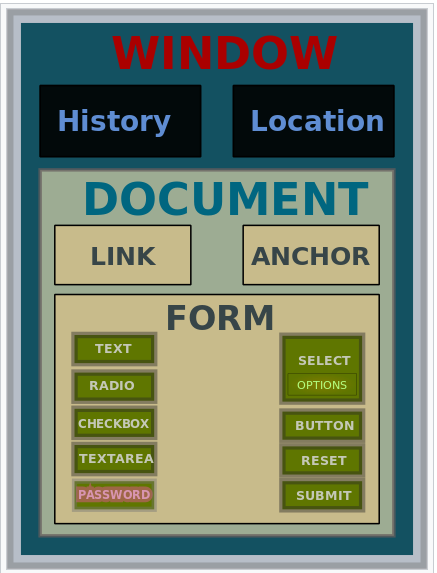
\includegraphics[scale=0.45]{images/dom-structure}
  \end{figure}

\end{frame}

\begin{frame}[fragile]
  \frametitle{Selektory DOM}
  \framesubtitle{Selektory}

  \verb|JavaScript| posiada wbudowane selektory drzewa DOM:

  \begin{itemize}
    \item \verb|getElementById(id)| --- zwraca element o podanym id
    \item \verb|getElementsByTagName(name)| --- zwraca listę elementów o podanym tagu
    \item \verb|getElementsByClassName(name)| --- zwraca listę elementów po podanej klasie
  \end{itemize}

\end{frame}


\begin{frame}[fragile]
  \frametitle{Selektory DOM}
  \framesubtitle{Selektory}

  Przykłady użycia zostaną przedstawione na podstawie następującegu kodu:

  \begin{minted}{html}
<html>
    <body>
        <h1 id="tytul">Witaj świecie</h1>
        <ol>
            <li class="czarny">Hello world</li>
            <li class="szary">Hallo Welt!</li>
            <li class="czarny">Bonjour le monde!</li>
        </ol>
    </body>
</html>
  \end{minted}

\end{frame}

\begin{frame}[fragile]
  \frametitle{Selektory DOM}
  \framesubtitle{Selektory}

  \begin{figure}
    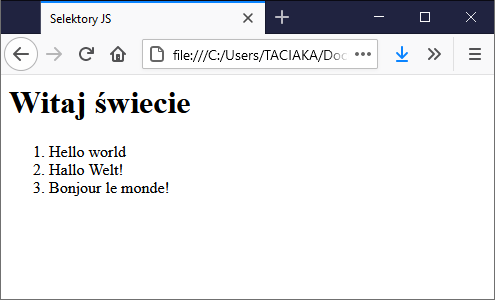
\includegraphics[scale=0.75]{images/dom-selectors-example}
  \end{figure}

\end{frame}


\begin{frame}[fragile]
  \frametitle{Selektory DOM}
  \framesubtitle{Selektory}

  \verb|document.getElementById(id)| --- zwraca obiekt o podanym identyfikatorze lub \verb|null|

  \begin{minted}{js}
let naglowek = document.getElementById('tytul');
  \end{minted}

  \begin{figure}
    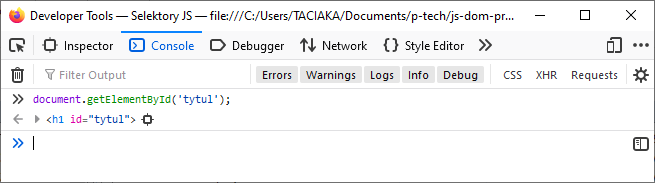
\includegraphics[scale=0.55]{images/dom-selector-getelementbyid}
  \end{figure}

\end{frame}


\begin{frame}[fragile]
  \frametitle{Selektory DOM}
  \framesubtitle{Selektory}

  \verb|document.getElementsByClassName(name)| --- zwraca listę obiektów o podanej klasie lub pustą listę

  \begin{minted}{js}
let czarne = document.getElementsByClassName('czarny');
  \end{minted}

  \begin{figure}
    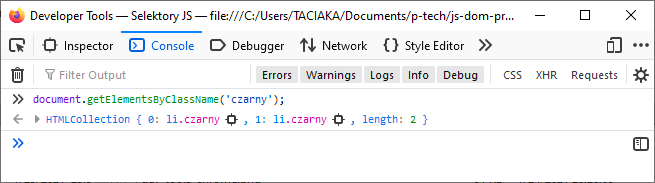
\includegraphics[scale=0.55]{images/dom-selector-getelementsbyclassname}
  \end{figure}

\end{frame}


\begin{frame}[fragile]
  \frametitle{Selektory DOM}
  \framesubtitle{Selektory}

  \verb|document.getElementsByTagName(name)| --- zwraca listę obiektów o podanym tagu lub pustą listę

  \begin{minted}{js}
let elementy = document.getElementsByTagName('li');
  \end{minted}

  \begin{figure}
    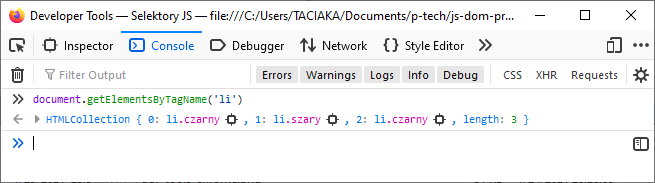
\includegraphics[scale=0.55]{images/dom-selector-getelementsbytagname}
  \end{figure}

\end{frame}


\begin{frame}[fragile]
  \frametitle{Selektory DOM}
  \framesubtitle{Obiekt HTMLElement}

  W zasadzie do czego przyda się zwracany element?

  Selektory zwracają obiekt \verb|HTMLElement| lub \verb|HTMLCollection| które reprezentują elementy w kodzie \textbf{HTML}.

  \begin{itemize}
    \item przez zwrócony obiekt, można rozmawiać z elementem na stronie
    \item atrybuty obiektu są odwzorowaniem atrybutów w HTMLu
  \end{itemize}

\end{frame}


\begin{frame}[fragile]
  \frametitle{Selektory DOM}
  \framesubtitle{Obiekt HTMLElement}

  Przykład:

  Kod \textbf{HTML}
  \begin{minted}{html}
<h1 id="tytul">Witaj świecie!<h1>
  \end{minted}

Kod \textbf{JavaScript}
  \begin{minted}{js}
let element = document.getElementById('tytul');
console.log(element.innerText);
  \end{minted}

Wyjście w konsoli
  \begin{minted}{bash}
Witaj świecie
  \end{minted}

\end{frame}


\begin{frame}[fragile]
  \frametitle{Selektory DOM}
  \framesubtitle{Obiekt HTMLElement}

  Co \verb|HTMLElement| kryje w sobie:

  \begin{itemize}
    \item \verb|innerText| --- tekst przechowywany w elemencie
    \item \verb|innerHTML| --- HTML przechowywany w elemencie
    \item \verb|hidden| --- ukrycie elementu
    \item \verb|id| --- identyfikator elementu
    \item \verb|className| --- klasa elementu
    \item \verb|style| --- dostęp do stylu elementu
    \item \verb|value| --- wartość elementu (pola tekstowe)
  \end{itemize}

\end{frame}


\begin{frame}[fragile]
  \frametitle{Selektory DOM}
  \framesubtitle{Obiekt HTMLElement}

  A jak modyfikować styl elementu?

  Aby zrealizować poniższy styl:
  \begin{minted}{css}
#tytul {
  color: red;
  font-size: 20px;
}
  \end{minted}

Należy odwołać się do poszczególnych atrybutów:
  \begin{minted}{js}
let element = document.getElementById('tytul');
element.style.color = 'red';
element.style.fontSize = 20;
  \end{minted}

\end{frame}








